\documentclass[a4paper]{scrartcl}
\usepackage[utf8]{inputenc}
\usepackage[english]{babel}
\usepackage{graphicx}
\usepackage{lastpage}
\usepackage{pgf}
\usepackage{wrapfig}
\usepackage{fancyvrb}
\usepackage{fancyhdr}
\pagestyle{fancy}

\usepackage[colorlinks=true,linkcolor=violet]{hyperref}
\usepackage[figure]{hypcap} %jump to img instead of caption text

\def\code#1{\texttt{#1}}


% Create header and footer
\headheight 27pt
\pagestyle{fancyplain}
\lhead{\footnotesize{Network Programming, ID1212}}
\chead{\footnotesize{Homework 3: RMI Fileserver}}
\rhead{}
\lfoot{}
\cfoot{\thepage\ (\pageref{LastPage})}
\rfoot{}

% Create title page
\title{Homework 3: RMI Fileserver}
\subtitle{Network Programming, ID1212}
\author{Max Körlinge, korlinge@kth.se}
\date{29 November 2018}

\begin{document}

\maketitle


\section{Introduction}

\noindent The assignment was to develop a distributed application, in this case, a fileserver and client, where clients can upload, download, and delete files on the server. A client also has to be able to register and login to the server. If someone accesses your file while you are logged in as a client, you are notified by the server. All users can list and read (download) all files on the server, but file permissions can be set to disallow writing (in our case, deleting) a file by all users except the owner of the file. It was sufficient to handle metadata when uploading and downloading files, you did not have to send the contents of the files. There was an optional task to send content as well, which was not completed. The requirements on the program were:

\begin{itemize}
    \item The program must be designed using a layered architecture and object-oriented design principles.
    \item Communicate using only RMI (remote method invocation) between client and server.
    \item Only the server is allowed to register in an RMI registry.
    \item The server uses a database to keep records on each user and file in the catalog.
    \item No state or data must be stored on the client.
    \item Server can only send state, not complete parts of the user interface, so that the user interface is handled entirely by the client.
    \item The user interface must be informative, so the user knows what is going on.
\end{itemize}

The program was written in full by the author of this report, to complete the basic task. The optional task was not completed.

\section{Literature Study}

To prepare for this assignment, all video material provided by the course on RMI and database access was viewed together with the code of the sample programs. Important information was gathered on how to communicate in a distributed java program using RMI, and how to access the database using JDBC and JPA, and the advantages of each.

\section{Method}

\noindent The program was written in Java using the IntelliJ IDE. Maven was used to handle dependencies. MySQL was chosen as the DBMS, with JPA as connecting framework.

The timeline was as follows: first, make a preliminary layered design with skeleton methods in both client and server. This included writing a simple user interface console loop with the different commands that were going to be used in the client program. Then, setup the database tables and write the related JPA entities in the server program, and make sure the database connection works and is able to perform all necessary operations. Thirdly, write the components needed for a successful RMI call from client to server, and make sure one operation is working in full (in this case, the \code{register} operation was completed first). Next, write a file handler that can store files on disk. Last, but not least, implement all other operations one by one according to the specifications.

\section{Result}

\noindent The complete source code can be found at \href{https://github.com/fongie/Filehandler}{https://github.com/fongie/Filehandler}.

\begin{itemize}
    \item To meet the demand of object-oriented design principles, the program was preliminary structured in layers before coding began. All classes are well encapsulated, not revealing their inner parts to the outer world, and all classes have one cohesive purpose. Duplication of code was avoided as much as possible. Method calls are always made in a downward direction through the layers.

        The client consists of a classic \code{view-controller-model} architecture. The \code{view} handles the user interface only, logical calls are passed to the \code{controller} whose job it is to decide where to delegate that logic. Usually it is either directed to the server, or to the local file handler. The \code{model} contains that local file handler, the only logic that the client performs on its own computer.

        The server has several duties and thus it required more layers to function well. It consists of a \code{controller-model-integration-entities} architecture. Since it is customary to pass the server controller as the remote object, the \code{controller} layer is the entrypoint for clients. It exposes an API to clients, and then directs their requests to classes suited to their purpose. The \code{model} contains classes handling connected clients, and working with files. The \code{integration} layer has classes that work with the database. There is also a data layer, named \code{entities}, which contains the JPA entities that directly represent data in the database.

        There is also a \code{common} package which includes classes and interfaces that are shared between the client and server.

        Special care is taken in protecting the objects and preserving the object oriented design in a few places. One example is the \href{https://github.com/fongie/Filehandler/blob/master/common/common/ReadableFile.java}{ReadableFile} interface. Both the \code{FileData} class originating from a client uploading, and the \code{File} entity from the server, implement this interface and are sent as readable files when they are sent over the network, to ensure that a client does not change anything contained in a file entity after the fact, and vice versa. Another example is what might be labeled as a remote observer pattern, which is that the remote client object \href{https://github.com/fongie/Filehandler/blob/143ac2e6c4f62b801610bd51a0752c945b97d358/filehandler_client/src/main/java/view/UserInterface.java#L250}{Callback}, which implements a remote interface, is called upon way down in the layered architecture, by the server, when the server wants to \href{https://github.com/fongie/Filehandler/blob/master/filehandler_server/src/main/java/model/Client.java#L19}{print} something to the console of a client.
    
    \item All communication was to be made using RMI, and it is. The server controller \href{https://github.com/fongie/Filehandler/blob/master/filehandler_server/src/main/java/controller/ServerController.java#L18}{goes through the motions} to be a remote object and the client \href{https://github.com/fongie/Filehandler/blob/master/filehandler_client/src/main/java/controller/Controller.java#L164}{stores it} and can \href{https://github.com/fongie/Filehandler/blob/master/filehandler_client/src/main/java/controller/Controller.java#L131}{call} it as if it was part of its own program. The client also, as mentioned above, passes a remote object to the server which is \href{https://github.com/fongie/Filehandler/blob/master/filehandler_server/src/main/java/model/Client.java#L19}{called} to notify the client of actions taken. Network communication is not made by anything other than RMI.
    
    \item Only the server was allowed to \href{https://github.com/fongie/Filehandler/blob/master/filehandler_server/src/main/java/startup/StartServer.java}{register itself} in an RMI registry. The client does not, so this requirement was met.
    
    \item The server uses a database to store information about users and files using the JPA framework. Database rows are represented as \href{https://github.com/fongie/Filehandler/tree/master/filehandler_server/src/main/java/entities}{entities} and database calls are made through the data access objects (DAO) in the integration layer. To avoid duplicated code, all DAOs inherit the \href{https://github.com/fongie/Filehandler/blob/master/filehandler_server/src/main/java/integration/DAO.java}{DAO} class which contains methods common to all DAOs, mainly handling the starting of and commiting of database transactions. MySQL was chosen as the datastore.
    
    \item The client was not allowed to store data (other than downloaded files), and all data needed to be sent to and processed by the server. If you study the client's \href{https://github.com/fongie/Filehandler/blob/master/filehandler_client/src/main/java/controller/Controller.java}{controller}, you will see that no methods process any data but the data is sent to the server. The server then returns processed data or throws exceptions on faulty data, which are passed through RMI back to the client controller. This way, no data is stored on the client.
    
    \item The server was not allowed to send parts of the user interface such as strings. There is, in fact, not a single method in the \href{https://github.com/fongie/Filehandler/blob/master/filehandler_server/src/main/java/controller/ServerController.java}{ServerController} that returns a String back to the client, only booleans or \code{ReadableFile}s. This means that the requirement is met.

    \item The user interface had to be informative. All data sent from the server is converted into typed information in the client's console, easy to understand. In Figure 1 you can see a sample output of using the application. There, a user registers as "root" and tries most operations available. You also see what happens when another user, "max", accesses a file that the user owns, on the line "Server: Your file 'remotename.txt' was downloaded by max".

\end{itemize}

\begin{figure}[h!]
    \begin{center}
        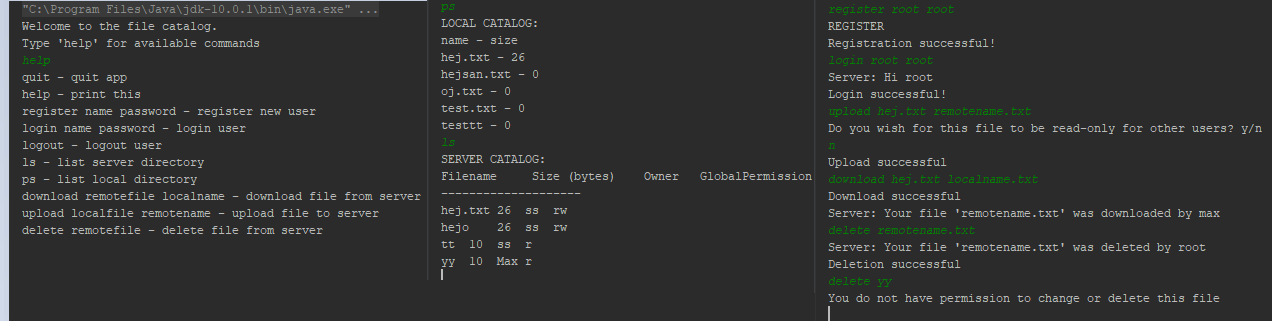
\includegraphics[scale=0.52]{ui.png}
        \caption{A sample output of the user interface}
        \label{fig:ui}
    \end{center}
\end{figure}



\section{Discussion}

This assignment was to develop a distributed application using RMI. The application was a file server, where a client can connect to and perform file operations on a remote catalog. Requirements concerned using RMI, using a database on the server side, not storing state on the client, having an informative user interface on the client, and structuring the program using object oriented design principles. All requirements were met and all functionality implemented. There was an optional task to send file contents using sockets, but this was not implemented due to time restraints.

Since I have not used RMI before, it was a learning experience and it took some time to get it to work the way I wanted it to. I have worked with databases in java before, so the JPA part was not very difficult.

The program could be improved mainly by implementing the optional task as well, which should not be too difficult, but circumstances have made it so that time right now is limited. You could also have a nice graphical interface to go with the program as well.


\section{Comments About the Course}

This was the most time consuming assignment so far, with a lot of lecture material and different integrating parts to work out. It unfortunately for me coincided with a big assignment in another course (Operating systems), and me working abroad during the weekends, so although I want to do the optional task because it is interesting and this assignment was very instructive, I can not do so in time.

I appreciate the way the course is structured, with large-ish practical programming tasks and no unnecessary time spent travelling to/from school due to recorded lectures, one of the best ways to learn in my opinion.

I spent quite a lot of time on this assignment but spread out over several days during some period of time, so it is difficult to pinpoint the exact hours. Probably around 5 hours on lecture material, 15-20 hours on the code and 3 hours on the report.

\end{document}
